\section{Methods}
The goal of this project is to train a model which as input takes the two-photon microscopy images of mice brains and outputs the locations of vescicles puncta. To train the model an annotated dataset is needed, where each puncta has been marked by hand by an expert in the field. The CNN is then trained by supervised learning to predict the location of the puncta. This section describes the methods used to achieve this.

\subsection{Preprocessing}
As the two-photon microscopy images comes in many different resolution depending on equipment used, preprocessing is needed to standardize the images. First all images have been scaled to the same resolution. Then, by finding the largest image, all other images has been padded with zeros until they achieve the same size. The images have then been resized to a size of 1024 by 1088. To ensure the masks still correspond to the images, the same scaling, padding and resizing have been applied to the masks. The images only have one colour channel with intensities between 0 and 4095. To make this match the input layer of the modified U-Net model, the intensities are normalized to be between 0 and 1 by first clamping all pixel intensities to be between 0 and 4095 and then dividing each pixel in the images with 4095. As the masks are binary to mark the location of puncta, this last preprocessing step has not been applied to the masks. The, in total, 722 images are now split into a training set of 506 images, a validation set of 104 images and a test set of 112 images. After the initial preprocessing the images have been resized to 512 by 544, that is the images have been halved. A bicubic interpolation has been used for the images and a nearest neighbour interpolation has been used for the masks in all datasets. Regardless of image sizes, in order to make the images comply with the modified U-Net model, three colour channels are needed. As our images only have one colour channel, this channel has simply been replicated twice.

\subsection{Models} \label{models}
The first model developed was a modified U-Net model where the encoder part has been replaced by a ResNet-18 model, transposed convolutions have been used for the upsampling layers to learn how the images are upsampled optimally, a sigmoid function have been used as activation function for the final output layer as the masks are binary, Adam have been used for optimization with an initial learning rate of 0.0001, soft DICE have been used for loss function and its weights have been initialized with the ImageNet weights. Very similarly, the second model uses the same configuration except it is not initialized with ImageNet weights. The last two models are LinkNet models using the same configurations as the previous two models.

% To determine whether pre-trained ImageNet weights should be used, an experiment was conducted early on in the project, where two models were trained using unmodified training data. The results of the training can be seen in \autoref{imagenet} where we see the model whose weights is initialized with the ImageNet weights performs better on the validation set. For this reason, the rest of the models trained are trained with the ImageNet weights.

%\begin{figure}
%	\centering
%	\begin{subfigure}[b]{0.48\linewidth}
%		\centering
%		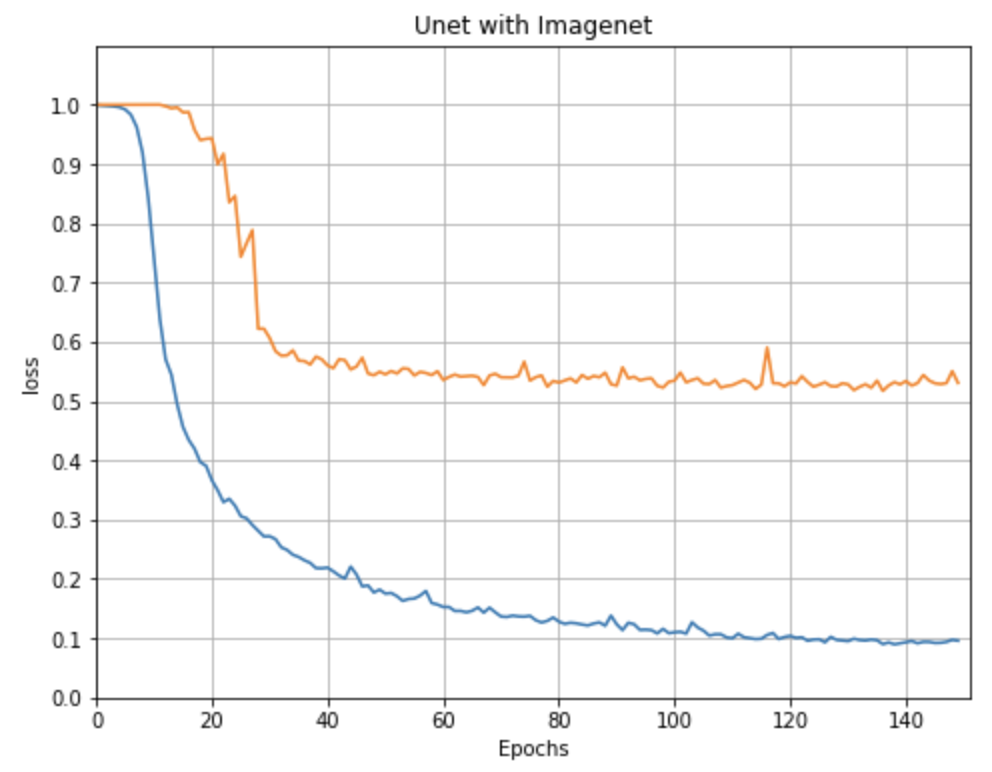
\includegraphics[width=\linewidth]{Materials/Method/UnetImagenet}
%		\caption{Model weights initialized with ImageNet weights.}
%	\end{subfigure}
%	\begin{subfigure}[b]{0.48\linewidth}
%		\centering
%		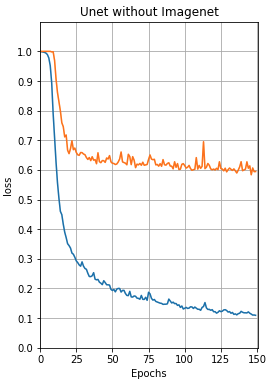
\includegraphics[width=\linewidth]{Materials/Method/UnetNoImagenet}
%		\caption{Model weights not initialized with ImageNet weights.}
%	\end{subfigure}
%	\caption{Both models are trained on unmodified training data. The blue graphs indicates training loss measured with DICE, and the orange graphs indicates validation loss also measured with DICE.}
%	\label{imagenet}
%\end{figure}

\subsection{Testing}
To measure the models unbiased performance on unknown data, the test set is used. As all predictions and true masks have image sizes 524 x 544 they are resized back to original sizes using the same interpolation rules. The 'immediate' output of the models are confidence maps, and to make these binary, we threshold them. This is done by thresholding all predicted masks from the training set and then computing the average DICE. The threshold that achieves the highest average DICE is then chosen, and all predicted masks from the test set are then thresholded by this value, and its unbiased performance can then be measured.\\
There exists different ways of measuring DICE on the test set. The test set can be split into three separate volumes, one for the single series images, one for the five series images and one for the six series images and the average DICE can then be measured across each. The three volumes can also further be split into 'time intervals' where the DICE is measured across all the images coming first in the series, second in the series and so on.

\subsection{Augmentations}
The first augmentation used is large random rotations. Here each of the original images have been rotated between $-45$ and $45$ degrees. Another dataset of small random rotations between $-30$ and $30$ degrees have also been created. The next augmentations flips each image horizontally and vertically giving us two more datasets. Two datasets have also been created for small and large random shearing in both the \textit{x} and \textit{y} direction. A \textit{mix} dataset has also been created where the original images were first sheared then rotated and finally flipped horizontally. A dataset was also created where the original images were 'bend' around the middle to form an arc shape. The last dataset created used the python package \textit{imgaug} to randomly apply one or more of the following augmentations to each image: horizontal flipping, vertical flipping, $80-120\%$ scaling, small translations, $-45$ to $45$ degrees rotations, $-16$ to $16$ degrees shearing, randomly drop $1-10\%$ of the pixels in the image, locally move some pixels around and lastly, perform local distortions. 

\subsection{Construction of augmented training sets}\label{construction}
With the augmented datasets, several training sets were constructed and used to train models. Each training set consists of 506 training images, and is constructed by randomly sample from the involved datasets without replacement, ensuring an even amount of images are taken from each dataset. An \textit{original} training set is also created consisting of the un-augmented images.